%%%%%%%%%%%%%%%%%%%%%%%%%%%%%%%%%%%%%%%%%%%%%%%%%%%%%%%%%%%%%%%%%
% !TEX root = interimreport.tex
\chapter{INTRODUCTION}\label{Ch1}
%%%%%%%%%%%%%%%%%%%%%%%%%%%%%%%%%%%%%%%%%%%%%%%%%%%%%%%%%%%%%%%%%
%%TODO INTRO YAZ


\section{Project Work Plan and Possible Updates}\label{plan}

%The table we presented in Form 3 is demonstrated in Table \ref{tab:work_plan} with updates. We completed the mac and SHLXOR \cite{Sairoglu} instructions earlier than expected and we consulted Prof. Örs Yalçın about our progress. We presented our work and since the instructions are not based on RISC-V, she advised us to change our instructions. She mentioned the Ibex processor which is a more stable core with RISC-V architecture and was extended in a past graduation project to support the ASCON encryption algorithm. We changed our instructions with compatible ones for the extended Ibex core. Convolution, deg, and AMB are replaced with ROT/ROTI and S-BOX instructions. Prof. Örs Yalçın also mentioned that the Ibex core is not able to implement the immediate rotation instruction and asked us to add the hardware. So our next tasks are implementing the S-BOX, ROT, and ROTI instructions on the LLVM compiler and adding the capability of immediate rotation to the Ibex processor. 

For the last months our main purpose was matching the S-BOX and ROT patterns. During our work, we found out that the LLVM RISC-V backend includes the ROT instruction as an extension. We enabled its flag and set its opcode. We are able to use the ROT instruction. How to enable the ROT instruction is explained in this form. Implementing S-BOX was challenging for us since it is a much more complicated than the other patterns we matched. Tablegen was not sufficent for our algorithm so we decided to match the pattern using c++ during the instruction selection phase. We started to build the algorithm in RISCVISelDAGToDAG.cpp file however we found out matching such a complex pattern is not quite reasonable. To implement s-box instruction, using intrinsic functions is a more preffered way because s-box algorithm is not a common pattern and the user may use it in different ways. It is also more practical way for the user so we decided to use intrinsics in s-box instruction. 

%\clearpage
\section{Purpose of Project}
Application Specific Instruction Set Processors (ASIPs) are becoming more popular with the development of embedded systems. The specialization of the core causes a tradeoff between flexibility and performance. For special purposes, using ASIPs increases efficiency, however, we can program a custom ASIP only by using assembly instructions that we defined. Programming custom processors with assembly language is not a preferred way of coding. We are also not able to use high-level languages because compiling tools are designed for common architectures with certain instructions. The ability to add custom instructions to compilers will enable us to make more use of custom hardware designs.

ASIPs are feasible for all application-specific embedded systems like consumer, industrial, automotive, home appliances, cryptology, medical, telecommunication, commercial, aerospace, and military applications. The custom backend that we will design under the supervision of Dr. Tankut Akgül, is going to serve the processor designed by Prof. Dr. Sıddıka Berna Örs Yalçın’s research team. When the project is completed, Prof. Yalçın is going to be able to produce the assembly codes that are compatible with the processor’s extended instruction set in addition to RISC-V.

There are two ways to avoid designing a specific compiler for embedded microprocessors. The first one is using a common processor that already has compiling tools. The advantage of it is reducing the costs for both hardware and software designs. However, it reduces efficiency dramatically because the processor is not designed for a specific task and hardware cost increases while the speed is decreasing. Another way is using an application specific instruction set processor and programming with the assembly instructions that the hardware designer defined. Theoretically, all efficiency benefits can be achieved but programming with assembly instructions increases coding difficulty excessively.

Prof. Yalçın and her team are studying on designing application specific instruction set processors. The purpose of this project is to create a compiler backend for a processor that supports custom instructions on top of RISC-V instructions. This compiler is going to help to program the custom processor by using high-level languages. Existing RISC-V compilers are not able to produce efficient assembly code for ASIPs. Therefore a need arose for a compiler backend.
The main reason for choosing this project is that we wanted to meet an actual need for a critical existing problem. The project has the potential to be the bridge between hardware and software of custom hardware projects in research, enabling them to be candidates for critical applications. Our team has skills and experience in low-level programming and digital design. Our project advisor Dr. Tankut Akgül’s lecture on microprocessors led us to work with him on the embedded systems. Our team member Mehmet Eymen Ünay is a double major student with computer engineering department. Bora İnan has experience in software development in the defense industry and Emrecan Yiğit is working on low-level robotics programming. Emrecan and Bora are taking digital system Design and application course from Prof. Yalçın to learn Verilog and get to know about hardware design. All of us have assembly, C, and FPGA programming experience. We also have worked with several open source frameworks on different Linux distros. We consider that our skills and experiences match the project we will be doing.

%\begin{table}
%    \centering
%    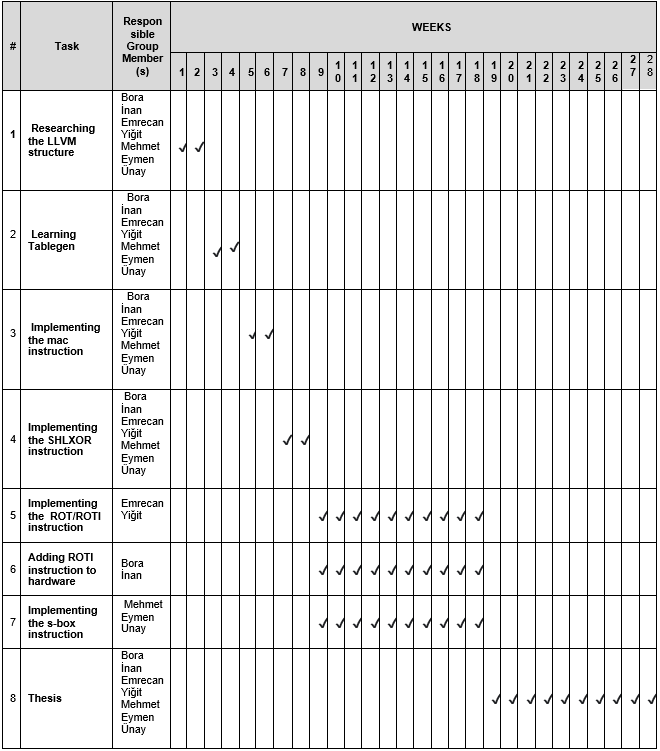
\includegraphics[width=\textwidth]{fig_general/work_plan.png}
%    \caption{Updated Work Plan}
%    \label{tab:work_plan}
%\end{table}
